\documentclass[../main.tex]{subfiles}
\graphicspath{ {../img/} }


\begin{document}


	\chapter{Part 2}


	\section{Why Rust?}


Rust is a multi-paradigm low level programming language which emphasizes memory safety, strict types and high performance. Despite its novel features(and associated learning curve),
such as variable ownership and its ommission of a null variable, it is already a loved language among developers, which forces the developer to write safer and more performant code.
Despite it lacking as many footguns as C/C++, it allows a great deal of control over what happens in a program. Though young, Rust is seen as the spearhead for the languages of the 
future, looking to replace C++ as the dominant low level language. Rust has been added to the Linux kernel, currently the only language to accompany C in this domain, and is being 
picked up by even the largest companies, such as Google. On the opposite side of the spectrum, hackers have begun writing in Rust, due to its aforementioned strengths and the 
current inability for malware scanners to detect threats in the binary[reference]. All of these reasons combined form our argument for learning Rust, which is what we had to do for
this project.

	\vspace{10pt}

	\section{Flow of the program}

	\subsection{Server code}

    \# server/src/main.rs

    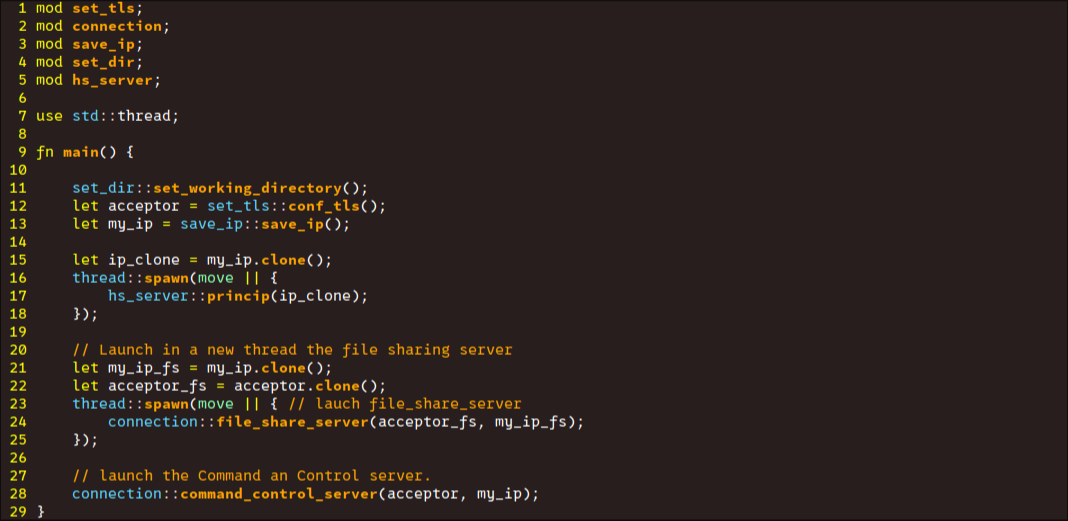
\includegraphics[width=450pt]{server_main.png}

    
	\vspace{10pt}

	\subsection{Client code}

    \# client/src/main.rs

    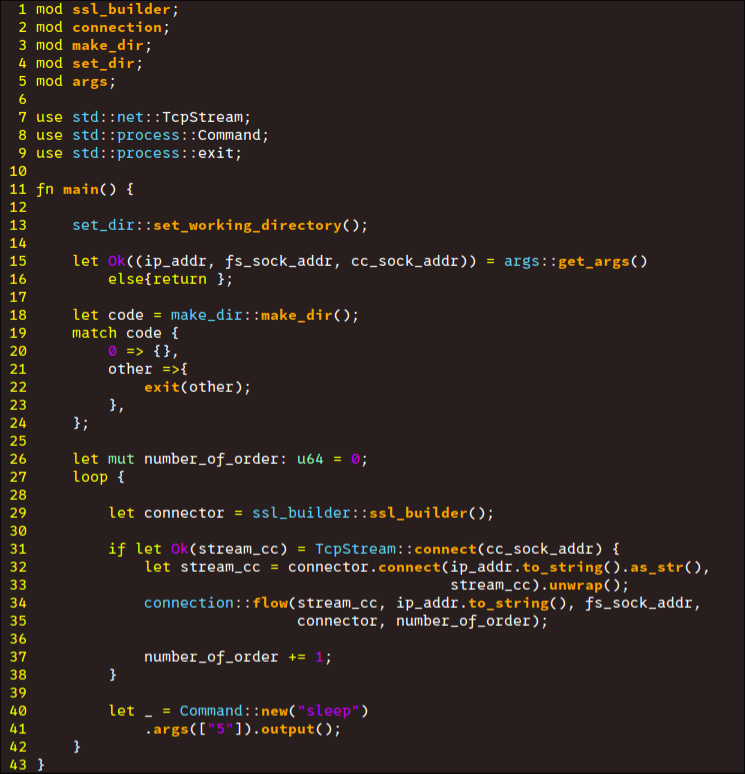
\includegraphics[width=450pt]{client_main.png}

    \# client/src/connection.rs

    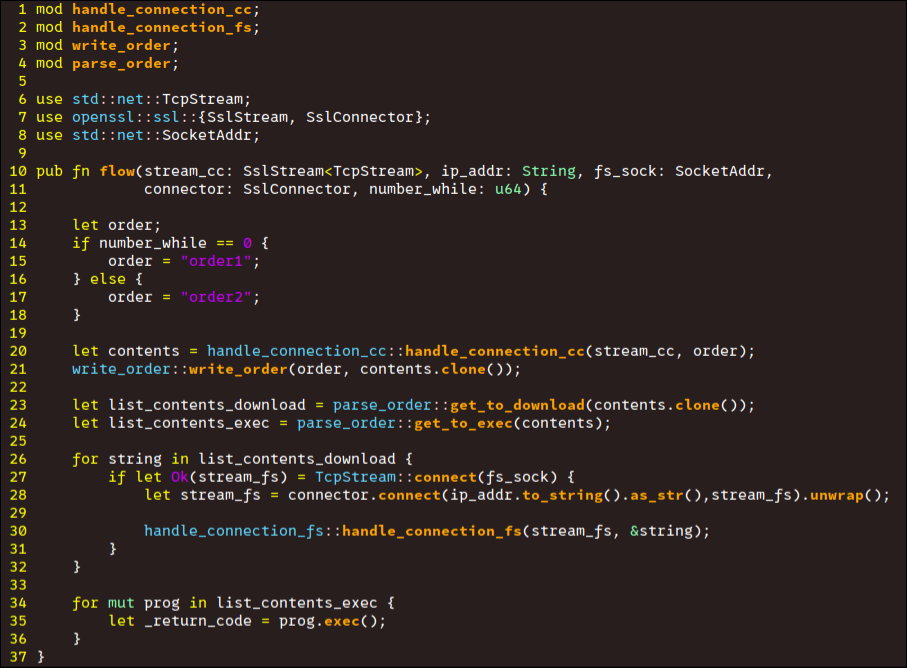
\includegraphics[width=450pt]{client_flow.png}

	\vspace{10pt}

	\section{Difficulties encountered while writting the program}



\end{document}
